\documentclass[10pt,a4paper]{article}
\usepackage[margin=1.8cm,top=1.65cm,bottom=1.7cm]{geometry}
\usepackage[T1]{fontenc}\usepackage{lmodern,microtype,booktabs,tabularx,array,graphicx,xcolor,amsmath,fancyhdr,xurl}
\usepackage[colorlinks=true,urlcolor=blue!60!black]{hyperref}
\definecolor{navy}{HTML}{173E56}\definecolor{teal}{HTML}{087F85}\definecolor{muted}{HTML}{586974}
\graphicspath{{../outputs/}}\setlength{\parindent}{0pt}\setlength{\parskip}{.35em}
\newcolumntype{Y}{>{\raggedright\arraybackslash}X}\renewcommand{\arraystretch}{1.16}
\setlength{\emergencystretch}{2em}\pagestyle{fancy}\fancyhf{}\setlength{\headheight}{15pt}
\fancyhead[L]{\small\color{muted}Business Intelligence / C2}\fancyhead[R]{\small\color{muted}Medina \& Castillo}
\fancyfoot[R]{\small\thepage}\renewcommand{\headrulewidth}{.3pt}
\newcommand{\heading}[1]{\vspace{.3em}{\large\bfseries\color{navy}#1}\par}
\begin{document}\thispagestyle{empty}
{\small\bfseries\color{teal} IIB423T-1 / C2 BRIEF}\par
{\LARGE\bfseries Monthly customer purchase profiles}\par
{\color{muted}Mois\'es Medina and Ignacia Castillo\hfill 8 November 2026}\par
\heading{1. Question and continuity}
Can monthly purchase frequency and invoice size distinguish useful customer profiles beyond a simple value-only grouping rule? We choose descriptive clustering to support a proposed month-end account review. W2 found that 430 of 4,293 identified customers contributed 60.5\% of identified annual purchase value, with IDs covering 85.7\% of eligible value. That ranking measures contribution but does not distinguish more invoices from larger invoices.

We reuse UCI Online Retail and W2's unchanged complete-month extract: 516,384 invoice lines, December 2010--November 2011. A source line is an item entry on an invoice. Our \textbf{modeling row is one active identified CustomerID-month}; recurring IDs are intentional. Accounts without an eligible identified purchase in a month do not become artificial zero records.

\textbf{W2 feedback response.} The received W2 hand-in lacked executable evidence and version links. C2 now includes an executed notebook with all project functions inline, readable outputs and a source link. We also follow an earlier fixed account group into later months and keep unidentified value separate. The ZIP contains only that notebook, this three-page brief and the presentation, following the updated C2 format.

\heading{2. Preparation and evaluation records}
Purchases require positive quantity/price, no C prefix and a provisional five-digit item code with an optional final letter. We retain every source row, keep exact repeats as in W2, and do not impute IDs or prices. Missing IDs stay in value coverage but cannot enter either customer grouping. The code pattern is a scope assumption, not a verified commercial category.

\begin{tabularx}{\linewidth}{@{}Yrrr@{}}
\toprule\textbf{Period} & \textbf{Source lines} & \textbf{Active ID-months} & \textbf{Unique active IDs} \\ \midrule
Train: Dec--Jul & 285,421 & 7,195 & 3,145 \\
Validation: Aug--Sep & 85,510 & 2,192 & 1,769 \\
Test: Oct--Nov & 145,453 & 3,021 & 2,405 \\
\bottomrule\end{tabularx}

Test is reserved first; validation comes from the earlier development pool. No invoice or ID-month crosses partitions. Shared CustomerIDs mean these are not independent new-customer populations. All periods were explored in earlier EDA: the later assessment is retrospective, not pristine prospective evidence.

\heading{3. First model and reference}
For each ID-month, $F$ is the number of distinct eligible invoices and $A$ is eligible purchase value per invoice (GBP). Monthly value is $F\times A$; adding it as a third clustering input would repeat the information. Inputs are available only after the month's invoices are recorded. This is grouping, not a forecast.

We apply $\log(1+x)$ to $F$ and $A$, then fit StandardScaler and KMeans \textbf{only on 7,195 training ID-months}. Logarithms reduce the influence of large ranges, and scaling prevents GBP from dominating counts. Large accounts remain. Settings are fixed: $k=3$, 20 initializations, 300 maximum iterations, Lloyd updates and seed 4232026. Three groups are a manageable first description, not an estimated optimal $k$.

The reference groups monthly value using training percentiles: lower up to \pounds{}329.65, middle up to \pounds{}1036.768, and higher above that cutoff. Both methods keep their learned rules fixed for validation and test. Validation checks finite inputs, complete assignments, populated groups and invariant fitted parameters before test assessment. No test result selects settings.

\newpage
\heading{4. Results on the same 3,021 test ID-months}
The test contains 2,405 distinct active IDs across October--November. A person can appear in both months and can change profile, so group sizes count ID-month records rather than permanent customer types.

\begin{tabularx}{\linewidth}{@{}Yrrrrr@{}}
\toprule\textbf{KMeans profile} & \textbf{Records} & \textbf{Share} & \textbf{Median $F$} & \textbf{Median $A$ (GBP)} & \textbf{Median monthly GBP} \\ \midrule
Profile 1 & 864 & 28.6\% & 1 & 152.48 & 155.31 \\
Profile 2 & 1,352 & 44.8\% & 1 & 416.19 & 416.19 \\
Profile 3 & 805 & 26.6\% & 2 & 313.23 & 733.09 \\
\bottomrule\end{tabularx}
The $A$ column is the median of each ID-month's average eligible invoice value. Separately calculated group medians need not multiply to median monthly value. Profile 1 has smaller invoices; Profile 2 mostly has one larger invoice; Profile 3 has more frequent purchases. Those descriptions follow observed medians, not known labels such as loyal or profitable.

\begin{center}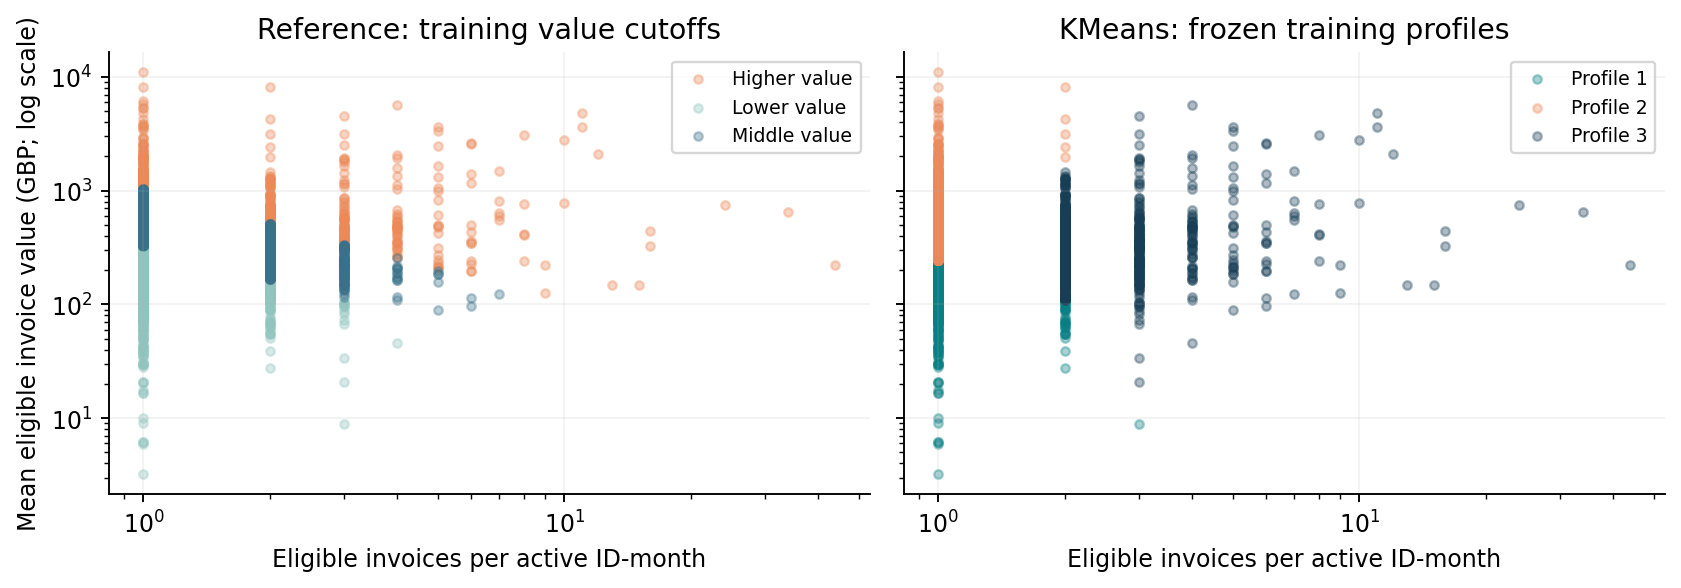
\includegraphics[width=\linewidth]{reference_vs_profiles.png}\end{center}
{\small Each point is an active identified test ID-month. Axes use logarithms; all records remain. Left: the fixed training-value reference. Right: the frozen KMeans assignment.}

\begin{tabularx}{\linewidth}{@{}YYY@{}}
\toprule\textbf{Internal separation metric} & \textbf{Validation: KMeans / reference} & \textbf{Test: KMeans / reference} \\ \midrule
Silhouette & 0.472 / 0.300 & 0.464 / 0.289 \\
\bottomrule\end{tabularx}
Silhouette compares within-group distances with distances to the nearest other group; larger values indicate clearer separation in this scaled feature space. Both methods use identical evaluation records and inputs. It is \textbf{not classification accuracy}, and there are no target labels. KMeans optimizes a related distance objective, so this advantage does not establish better commercial outcomes.

The reference's higher-value group contains 380 test ID-months (12.6\%); its share need not remain 10\% because the training cutoff stays fixed. Of those 380 records, 124 fall in Profile 2 and 256 in Profile 3. Thus high recorded value can reflect different purchase patterns. The notebook includes the complete cross-table and both sets of profiles.

Profile 3 represents 26.6\% of test ID-months and 55.0\% of identified test value. This supports examining its accounts and invoices, while the value-only rule remains a simpler option when contribution alone is the question. Neither description estimates profit or an intervention effect.

\newpage
\heading{5. Later account contribution and unidentified value}
Using December--September records only, we freeze the highest-value 362 of 3,613 known IDs and follow that same review group later. This addresses the instructor's stability question. Its size differs from each monthly top decile, so the table is a persistence diagnostic, not a like-sized model contest.

\begin{tabularx}{\linewidth}{@{}YYYYY@{}}
\toprule\textbf{Later month} & \textbf{Frozen IDs active} & \textbf{Frozen group / known value} & \textbf{Re-ranked K10} & \textbf{Unidentified / all value} \\ \midrule
2011-10 & 218 / 362 & 48.16\% & 50.77\% & 8.94\% \\
2011-11 & 265 / 362 & 46.13\% & 47.79\% & 21.45\% \\
\bottomrule\end{tabularx}
The earlier review group continues to contribute substantial identified value, with varying activity. Missing purchases in one later month do not establish churn. Different coverage and account mixes prevent attributing the change to one cause.

\begin{tabularx}{\linewidth}{@{}Yrr@{}}
\toprule\textbf{Share of all eligible value} & \textbf{October} & \textbf{November} \\ \midrule
Known top-decile purchases & 46.24\% & 37.54\% \\
Other identified purchases & 44.83\% & 41.01\% \\
Unidentified purchases & 8.94\% & 21.45\% \\
\bottomrule\end{tabularx}
Each month's three shares sum to 100\% before rounding. Unidentified value may belong to many people and is never treated as one customer or one cluster. In November, 21.45\% of eligible value is outside customer profiling. The annual 60.5\% K10 and these monthly shares have different windows and denominators.

\heading{6. Model verdict, limit and improvement}
\textbf{Model verdict.} Retain this first model for descriptive profiling. It assigns all later records to three interpretable groups. Test silhouette 0.464 exceeds the value rule's 0.289 and is close to validation 0.472. This supports describing the selected purchase patterns; commercial usefulness remains unvalidated. There is no universal silhouette pass mark or pristine prospective test.

\textbf{Proposed use.} Structure manual account review with the profiles and investigate ID capture. Retain the simple value rule when contribution alone is the question. Automated actions and campaign effects require further evidence.

\textbf{Important limits.} The profiles cover purchase-active identified historical records. Missing identities, provisional item codes, repeated participation and varying month lengths limit interpretation. KMeans imposes three Euclidean groups and depends on the chosen scaling/features. Previous full-period exploration limits any claim of untouched testing. We do not establish current market behavior, permanent segments, future loss or causal effects.

\textbf{Next improvement.} Obtain recent transactions and verified customer linkage, apply the frozen rule to comparable complete months, and review profile usefulness with a commercial stakeholder. That would provide evidence beyond this already-explored historical period.

\textbf{Agreed review roles and AI.} Mois\'es: data, features, model and evaluation; Ignacia: profiles, reference comparison and business conclusions. Both: question, methodology, final review and presentation. Codex assisted with code/text/layout drafts and automated checks. Each member remains responsible for reviewing and explaining the work.

\heading{References and submitted evidence}
{\small
Chen, D. (2015). \emph{Online Retail}. UCI Machine Learning Repository. \href{https://doi.org/10.24432/C5BW33}{doi:10.24432/C5BW33}. CC BY 4.0.\par
scikit-learn 1.5.2: \href{https://scikit-learn.org/1.5/modules/generated/sklearn.cluster.KMeans.html}{KMeans}, \href{https://scikit-learn.org/1.5/modules/generated/sklearn.preprocessing.StandardScaler.html}{StandardScaler}, \href{https://scikit-learn.org/1.5/modules/generated/sklearn.metrics.silhouette_score.html}{silhouette score}.\par
Fontecilla, T. (2026). \emph{C2: Train and explain your first model}, updated IIB423T-1 brief; course notebooks on clustering and validation.\par
Executed evidence: \path{01_C2_Customer_Profiles.ipynb}. Presentation: \path{GROUP_Medina_Castillo_C2_Presentation.pptx}. \href{https://github.com/DirtyCheese02/online-retail-bi-medina-castillo/tree/c2-roles-2026-11-08}{Versioned project repository}. The ZIP contains only notebook, brief and presentation.
}
\end{document}
